\chapter{Synchronisation, Mutexes and Deadlocks}

A Distributed System consists of a collection of distinct processes 
that are spatially separated and run concurrently. In systems with multiple concurrent processes, it is economical to share the system resources. This sharing may be \textit{cooperative} or \textit{competitive}.

Both competitive and cooperative sharing require adherence to 
certain rules of behavior that guarantee that correct interaction 
occurs. The rules of enforcing correct interaction are implemented in the 
form of synchronization mechanisms. 

In single CPU systems, synchronization problems such as mutual exclusion can be solved using semaphores and monitors. These methods rely on the existence of shared memory.

We cannot use semaphores and monitors in distributed systems since two processes running on different machines cannot expect to have shared memory. Even simple matters such as determining one event happened before the other event requires careful thought.

In distributed systems, it is usually not possible or desirable to collect all the information about the system in one place and synchronization among processes is difficult due to the following 
features of distributed systems:

\begin{itemize}
\item The relevant information is scattered among multiple machines.
\item Processes make decisions based only on local information.
\item A single point of failure in the system should be avoided.
\item No common clock or other precise global time source exists. 
\end{itemize}

\section{Clocks}
Why do we want to distribute the current time across the system? There are external reasons; we often want to measure time accurately:
\begin{itemize}
\item For billings: How long was computer X used? 
\item For legal reasons: When was credit card W charged? 
\item For traceability: When did this attack occurred? Who did it? 
\end{itemize}
To achieve this, the system must be in sync with an external time reference; this is usually the world time reference UTC (Coordinated Universal Time).

There are also internal reasons; many distributed algorithms use time:
\begin{itemize}
\item Kerberos (authentication server) uses time-stamps 
\item Internal time can be used to serialise transactions in databases 
\item Internal time can be used to minimise updates when replicating data 
\end{itemize}
To achieve this, the system must be synchronised internally; this \textit{does not} require synchronisation to an external time reference!

Time is unambiguous in a centralised system. A process can always make a system call to know the time; if two processes $A$ and $B$ are running on the same system and $B$ requests the current time $B_{time}$ after $A$ requests $A_{time}$, then it is guaranteed that $B_{time} > A_{time}$.

However, this is not the case in a distributed system. If the two processes are on different machines, $B_{time}$ may not be greater than $A_{time}$.

In general, human-made clocks are imperfect. They run slower or faster than "real" physical time. The amount of variation from "real time" is called the \textit{drift}; a drift of 1\% implies that the clock gains or loses a second every 100 seconds.

This can be quantified. If the real time is $t$, the measured time value of a clock is $C_p(t)$, and the maximum drift rate allowable is $\rho$, a clock can be said to be non-faulty \footnote{It is always assumed that any clock has some amount of drift. The nature of physics makes it implausible that a "perfect" clock will ever exist.} if the following condition holds:
\[ 1 - \rho \le \frac{dC}{dt} \le 1 + \rho \]

\subsection{Cristian's Algorithm}
\textit{Cristian's algorithm}, as depicted in \autoref{fig:screenshot028}, synchronizes the clocks of all other machines to the clock of one machine, the \textit{time server}. If the clock of the time server is adjusted to the real time, all the other machines are synchronized to the real time.

Every machine requests the current time to the time server. The time server responds to the request as soon as possible. The requesting machine sets its clock to
\[ C_s + \frac{T_1 - T_0 - I}{2} \]

To avoid clocks moving backwards for any machine, a clock adjustment must be introduced gradually.

\begin{figure}
\centering
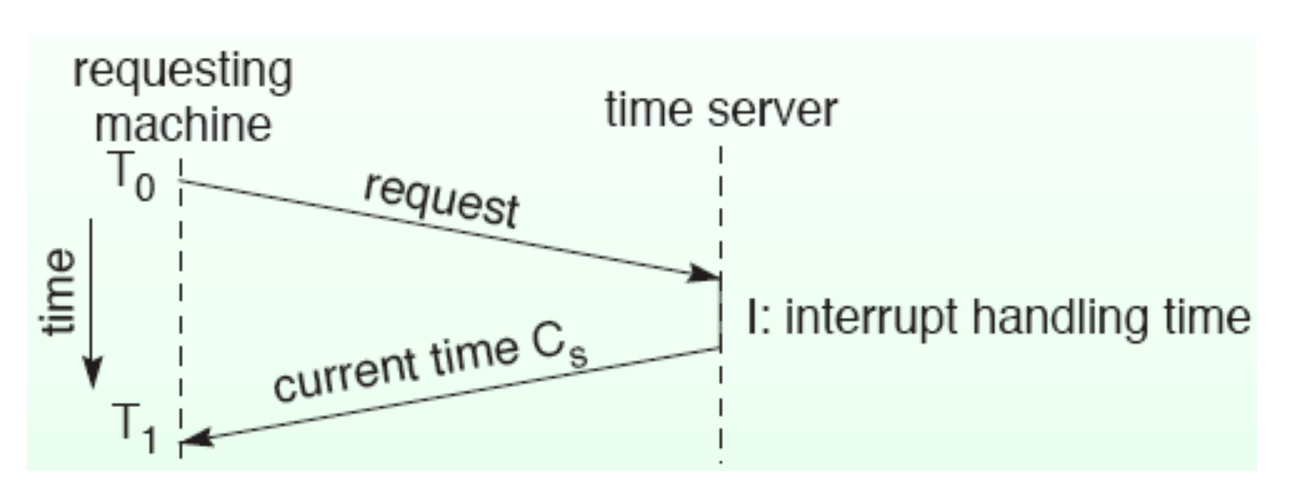
\includegraphics[width=0.7\linewidth]{screenshot028}
\caption{Cristian's algorithm for clock synchronisation.}
\label{fig:screenshot028}
\end{figure}

\subsection{Berkeley Algorithm}
The \textit{Berkeley algorithm}, as developed by Gusella and Zatti, uses a master server that communicates with its slaves to determine the time offset to be applied to each slave. It is illustrated in \autoref{fig:screenshot029}.

The complete algorithm generally follows these steps:
\begin{itemize}
\item A master server is chosen with a ring-based election algorithm (Chang and 
Roberts algorithm). 
\item The master polls the slaves who reply with their time in a similar way to Cristian's algorithm.
\item The master observes the round-trip time (RTT) of the messages and estimates the time of each slave and its own.  
\item The master then averages the clock times, ignoring any values it receives far outside the values of the others. 
\item Instead of sending the updated current time back to the other process, the master
 then sends out the amount (positive or negative) that each slave must adjust its clock. This avoids further uncertainty due to the RTT of the slave processes.  
\item Everybody adjusts their times appropriately.
\end{itemize}

\begin{figure}
\centering
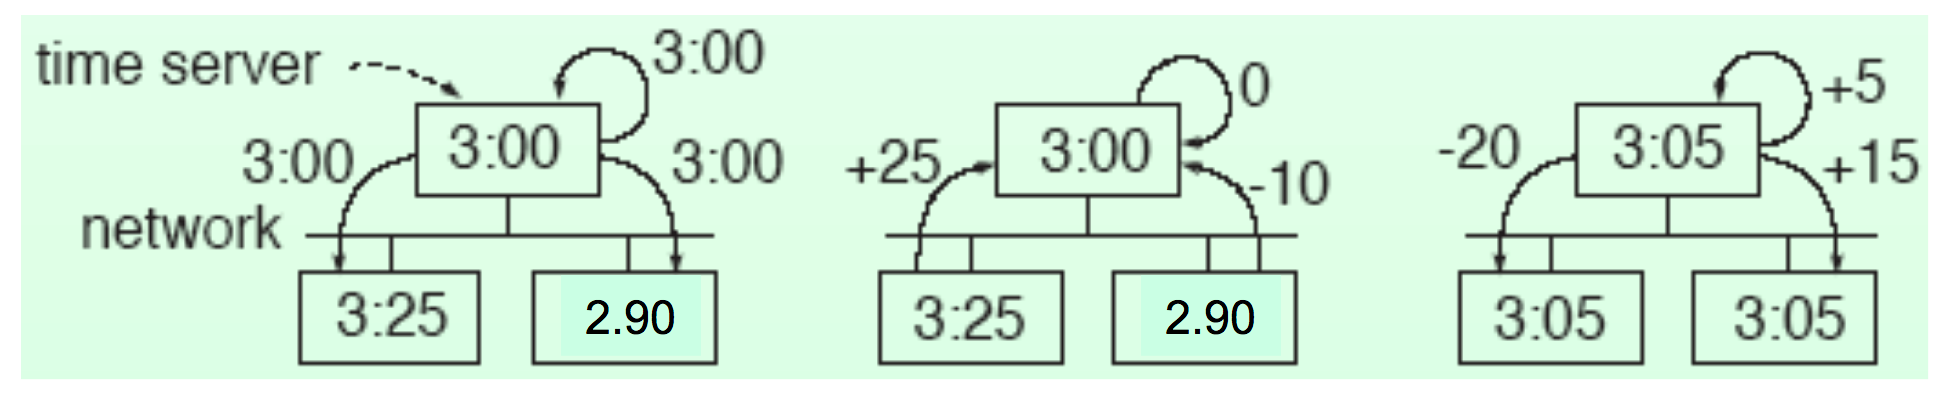
\includegraphics[width=0.7\linewidth]{screenshot029}
\caption{The Berkeley algorithm for clock synchronisation.}
\label{fig:screenshot029}
\end{figure}

The use of an average cancels out the tendency of individual clocks to drift, addressing one of the major shortcomings of Cristian's algorithm.

However, special consideration must be given to avoiding direct application of a negative clock alteration. Computers generally rely on \textit{monotonic time}, in which the clock value must either stay the same or go forwards; it must never go backwards.

The simple solution is to halt the clock in the event of a negative clock alteration, so that time naturally synchronises to the alteration required. However, this may cause issues of its own (as time is effectively stopped). For minor corrections, most systems will prefer to slow the clock (known as \textit{clock skew}), so that the correction is distributed across a longer period of time.

\subsection{Averaging Algorithm}
Both Cristian's algorithm and the Berkeley algorithm are centralized algorithms with disadvantages including the existence of a central point of failure and high traffic volume around the server.

The \textit{averaging algorithm} is a decentralized algorithm. It divides time into resynchronization intervals with a fixed length \textit{R}. Every machine broadcasts the current time at the beginning of each interval according to its clock. A machine collects all other broadcasts for a certain interval and sets the local clock by the average of their arrival times. 

\begin{figure}
\centering
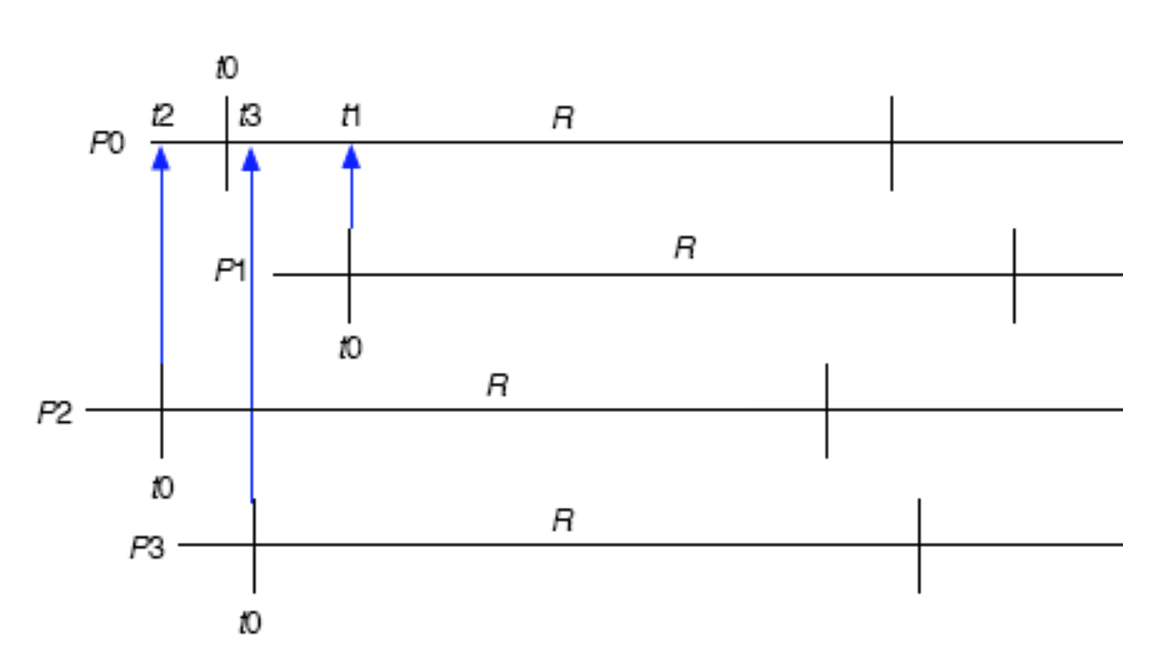
\includegraphics[width=0.7\linewidth]{screenshot030}
\caption{An example of the averaging algorithm for clock synchronisation.}
\label{fig:screenshot030}
\end{figure}

\autoref{fig:screenshot030} depicts an example of the averaging algorithm for a system with four nodes. The clock on processor $P0$ should be advanced in accordance with the increment $\delta t_0$:
\[ \delta t_0 = \frac{t_0 + t_1 + t_2 + t_3}{4} - t_0 \]

\subsection{Lamport's Synchronisation Algorithm}
Leslie Lamport showed that clock synchronisation need not be absolute. If two processes do not interact, they do not need synchronised clocks. All that matters is that processes agree on the order in which events occur.

Based on this, it can be said that there are two types of clocks: \textit{physical clocks} and \textit{logical clocks}. Physical clocks agree on time within a certain time limit; the previous synchronisation algorithms attempt to synchronise physical clocks.

Logical clocks are based on the assumption that the time itself is irrelevant for many purposes; all that matters is that all processes agree on some time value that can be used to determine the sequence in which events occur. This time value \textit{does not need to be the real time}.

Lamport's algorithm is used to determine the ordering of events. This is done by establishing the happens-before relation (see \autoref{sssec:causalordering}). Note that if two events $X$ and $Y$ occur in different processes that do not interact (even indirectly), then neither $X \rightarrow Y$ and $Y \rightarrow X$; these events occur \textit{concurrently}.

The goal of the algorithm is to assign a time value $C(A)$ for which all processes agree on for any event $A$. This time value must obey $A \rightarrow B \implies C(A) < C(B)$ and that $C(A)$ \textit{always} increases and can never decrease.

If event $A$ happens before event $B$ within the same process, $C(A) < C(B)$ is satisfied. If event $A$ and event $B$ represent the sending and receiving of a message, the clock of the receiving side is set so that $C(A) < C(B)$. For all events, the clock is increased at least by 1 between two events.

The largest shortcoming of the Lamport clock is that while $a \rightarrow b \implies C(A) < C(B)$, $C(A) < C(B) \not\implies a \rightarrow b$. This means that causal dependencies cannot be derived from time stamps.

The cause of this behaviour is that clocks advance independently or from messages, but there is no way of recovering the impetus for a clock advancement.

\begin{figure}
\centering
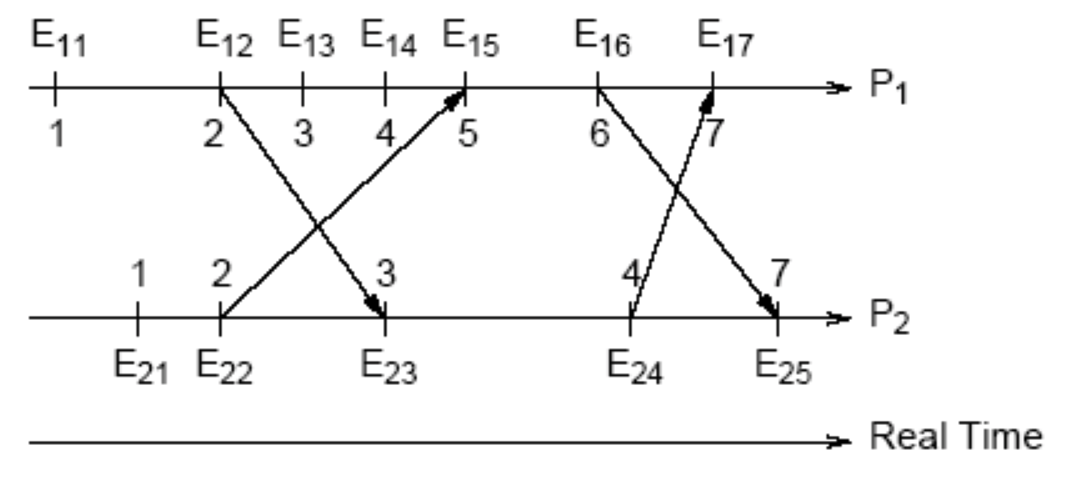
\includegraphics[width=0.7\linewidth]{screenshot031}
\caption{Illustration of the shortcoming with Lamport clocks.}
\label{fig:screenshot031}
\end{figure}

In \autoref{fig:screenshot031}, $E_{12} \rightarrow E_{23}$ implies that $C_1(E_{12}) < C_2(E_{23})$; however, it is possible that $E_{13} \not\rightarrow E_{24}$ even though $C_1(E_{13}) < C_2(E_{24})$.

This results in a partial ordering on events, which is insufficient for situations in which a total ordering is required (e.g. distributed locks).

\subsection{Vector Clock}
Each process $i$ maintains a vector clock $\mathbf{V}_i$ of size $N$, where $N$ is the number of processes. $\mathbf{V}_i[j]$ refers to process $i$'s knowledge of process $j$'s clock. The vector $\mathbf{V}_i[j]$ is initialised with $0$ for $i, j \in \{1, 2, \dots, N\}$.

The clocks are advanced in accordance with these steps:
\begin{enumerate}
\item Before process $i$ timestamps an event, it executes $\mathbf{V}_i[i] = \mathbf{V}_i[i] + 1$; that is, it increments its timestamp for itself.
\item When a message $m$ is sent from process $i$ to process $j$: \begin{itemize}
	\item Process $i$ executes $\mathbf{V}_i[i] = \mathbf{V}_i[i] + 1$ and sends $\mathbf{V}_i$ with $m$.
	\item Process $j$ receives $m$ and $\mathbf{V}_i$, and merges its own vector clock $\mathbf{V}_j$ with $\mathbf{V}_i$ using the following equation:
	\[ \mathbf{V}_j[k] = 
		\begin{cases} 
			\max(\mathbf{V}_j[k], \mathbf{V}_i[k]) + 1 & \text{if } j = k \text{ (as in scalar clocks)} \\
			\max(\mathbf{V}_j[k], \mathbf{V}_i[k]) & \text{otherwise} \\
		\end{cases}
	\]
\end{itemize}
\end{enumerate}

This guarantees that everything that occurs on process $j$ after $m$ is now causally related to everything that previously happened at process $i$.

This addresses the shortcoming of the Lamport clock as it can be used to establish whether a causal relationship exists or not. This is illustrated in \autoref{fig:screenshot032}, where each triple is the vector clock value at that instant for that process, and the red value is the corresponding scalar Lamport clock.

\begin{figure}
\centering
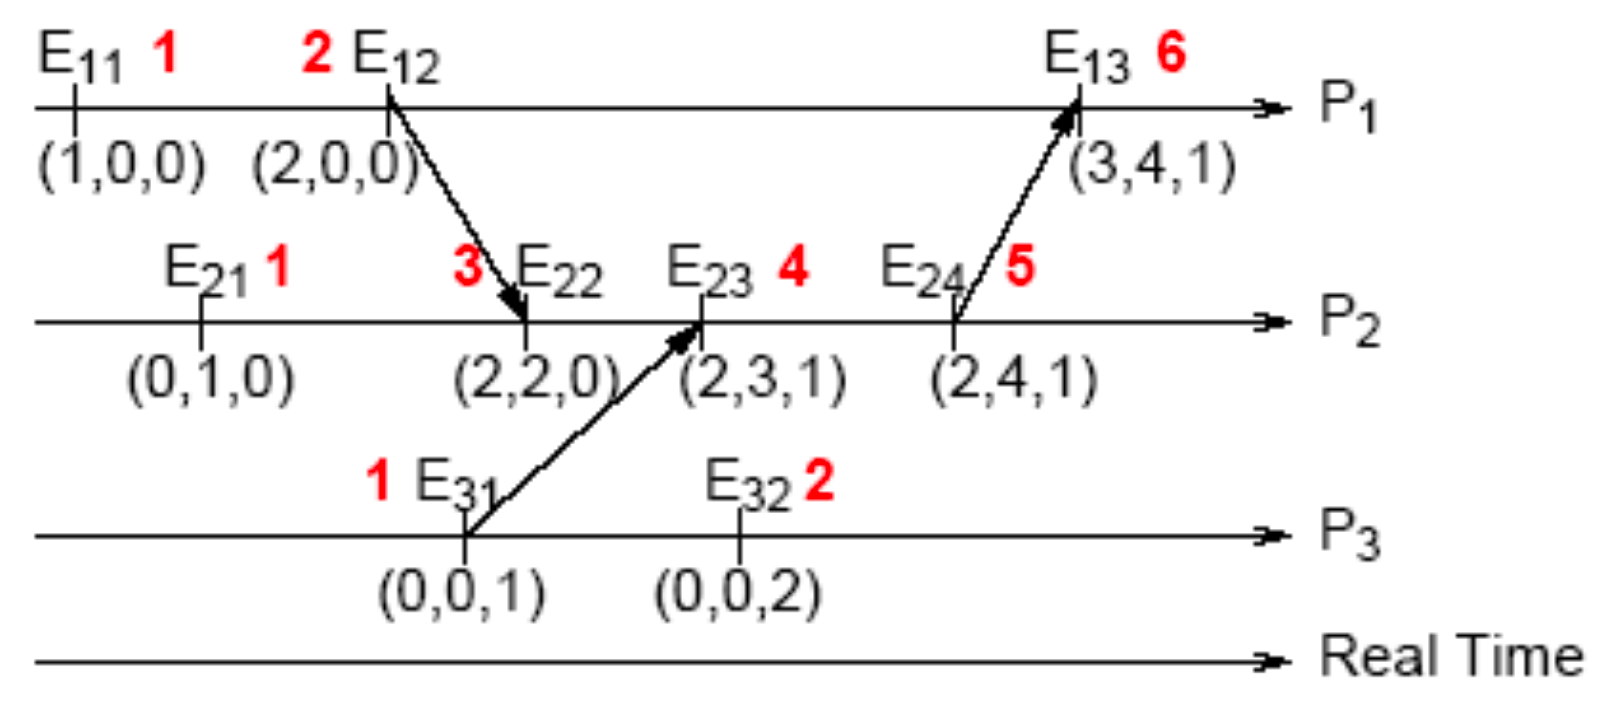
\includegraphics[width=0.7\linewidth]{screenshot032}
\caption{Vector clock compared to a Lamport clock.}
\label{fig:screenshot032}
\end{figure}


Note that $C_1(E_{12}) = C_3(E_{32})$, but the vector clocks $(2, 0, 0)$ and $(0, 0, 2)$ do not agree; this implies that these events are not causally related. Additionally, $C_2(E_{24}) > C_3(E_{32})$, but $(2, 4, 1) \not> (0, 0, 2)$ and thus $E_{32} \not\rightarrow E_{24}$.

\section{Mutual exclusion}
When multiple processes access shared resources, the concept of \textit{critical sections} is a relatively easy way to control access of the shared resources. Critical sections are sections in a program that access shared resources; these regions effectively act as gates that prevent other processes from accessing the resource until the process using the resource exits the region.

However, critical sections are implemented using semaphores and monitors in single-processor systems; these mechanisms do not generalise to distributed systems.

\subsection{Centralised Exclusion}
This algorithm, depicted in \autoref{fig:screenshot033}, simulates the behaviour of mutual exclusion in single processor systems. One process is elected as the coordinator. When a process wants to enter a critical section, it sends a request to the coordinator stating which critical section it wants to enter.

If no other process is currently in that critical section, the coordinator returns a reply granting permission. If a different process is already in the critical section, the coordinator 
queues the request. 

When the process exits the critical section, the process sends a message to the coordinator releasing its exclusive access. The coordinator takes the first item off the queue of deferred requests and sends that process a grant message.

\begin{figure}
\centering
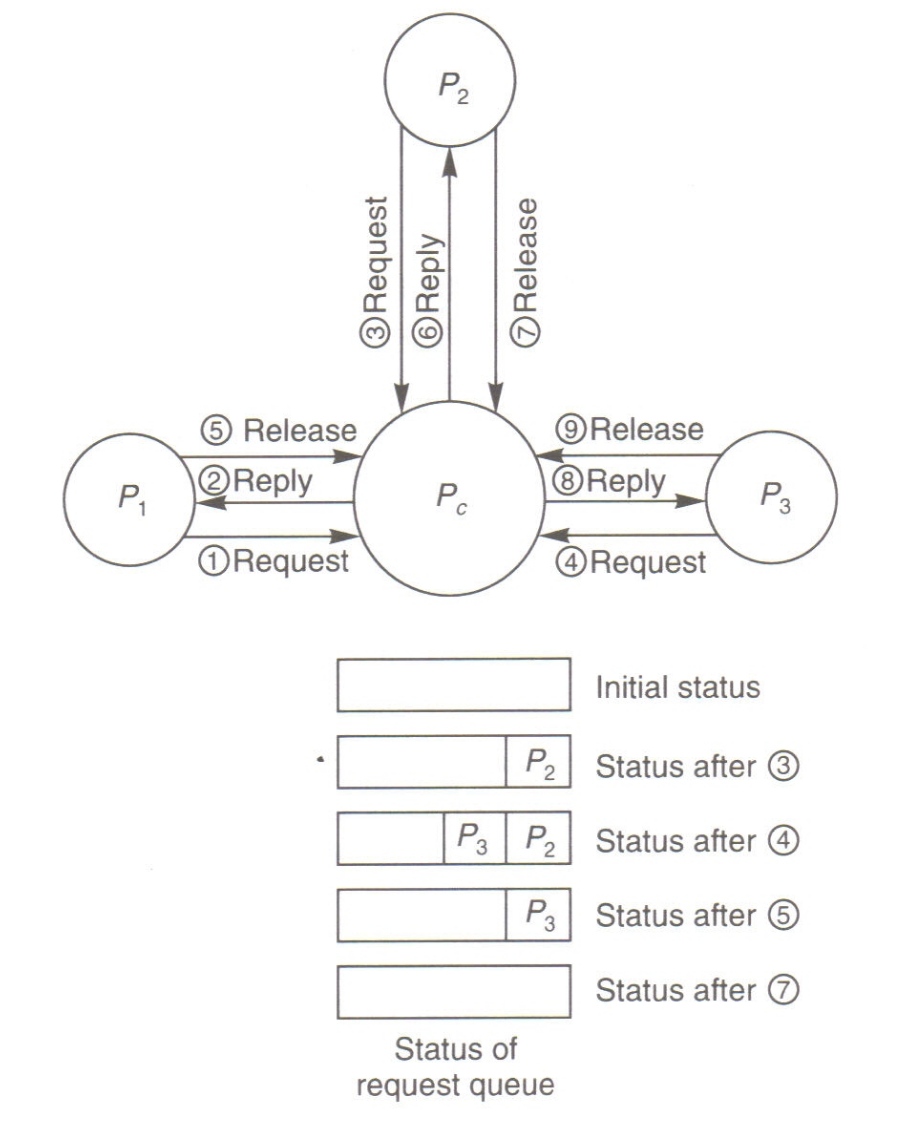
\includegraphics[width=0.7\linewidth]{screenshot033}
\caption{Centralised exclusion algorithm.}
\label{fig:screenshot033}
\end{figure}

The advantages of this system are: \begin{itemize}
\item Since the service policy is first-come first-serve, it is fair and no process waits forever.
\item It is easy to implement.
\item It requires only three messages, request, grant, and release, per use of a critical section.
\end{itemize}

The disadvantages of this system are: \begin{itemize}
\item If the coordinator crashes, the entire system may go down.
\item Processes cannot distinguish a dead coordinator from “permission denied.”
\item A single coordinator may become a performance bottleneck. 
\end{itemize}

\subsection{Distributed Algorithm}
Ricart and Agrawala's distributed algorithm, illustrated in \autoref{fig:screenshot034}, requires ordering of all events in the system, which can be provided using the Lamport clock.

When a process wants to enter a critical section, the process sends a request message to all other processes. The request message includes the name of the critical section, the process number, and the current time.

The other processes will then receive the request message. One of three things can happen: \begin{itemize}
\item If the process is not in the requested critical section and also has not sent  a request message for the same critical section, it returns an OK message to the requesting process.
\item If the process is in the critical section, it does not return any response and puts the request to the end of a queue.
\item If the process has sent out a request message for the same critical section, it compares the time stamps of the sent request message and the received message. If the time stamp of the received message is smaller than the one of the sent message, the process returns an OK message. If the time stamp of the received message is larger than the one of the sent message, the request message is put into the queue.
\end{itemize}

The requesting process waits until all processes return OK messages. When the requesting process receives all OK messages, the process enters the critical section.

When a process exits from a critical section, it returns OK messages to all requests in the queue corresponding to the critical section and removes the requests from the queue. Processes enter a critical section in time stamp order using this algorithm. 

\begin{figure}
\centering
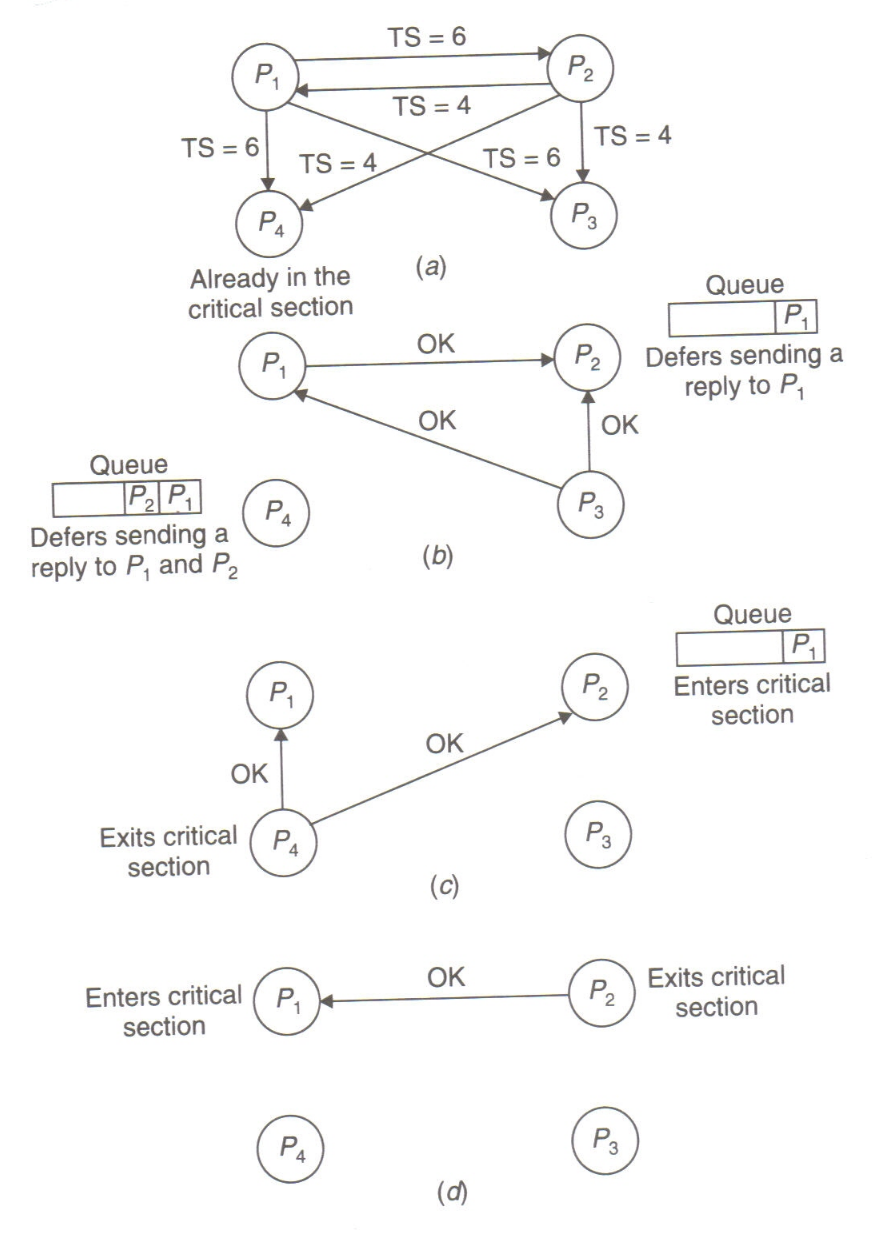
\includegraphics[width=0.7\linewidth]{screenshot034}
\caption{Distributed critical section algorithm.}
\label{fig:screenshot034}
\end{figure}

This algorithm will result in no deadlock or starvation, but is subject to a variety of disadvantages, listed here: \begin{itemize}
\item $2(n - 1)$ messages are required to enter a critical section, where $n$ is the number of processes.
\item If one of the processes fails, it will not respond to the request. No process will thus be able to enter the critical section.
\item In a centralised system, the coordinator is the bottleneck. As all processes send requests to all other processes in this system, \textit{all} processes are bottlenecks.
\end{itemize}

\subsection{Token Ring Algorithm}
The token ring algorithm, seen in \autoref{fig:screenshot035}, constructs a virtual ring by assigning a sequence number to each process. This can be done even if the processes are not physically connected in a ring shape; process $0$ receives a token when the ring is initialised.

The token is passed to the process with the next sequence number. A process can enter the critical section only if the process holds the corresponding token. The process passes the token to the next process when it is done. A process passes the received token if it does not need to enter the critical section upon receiving the token. 

\begin{figure}
\centering
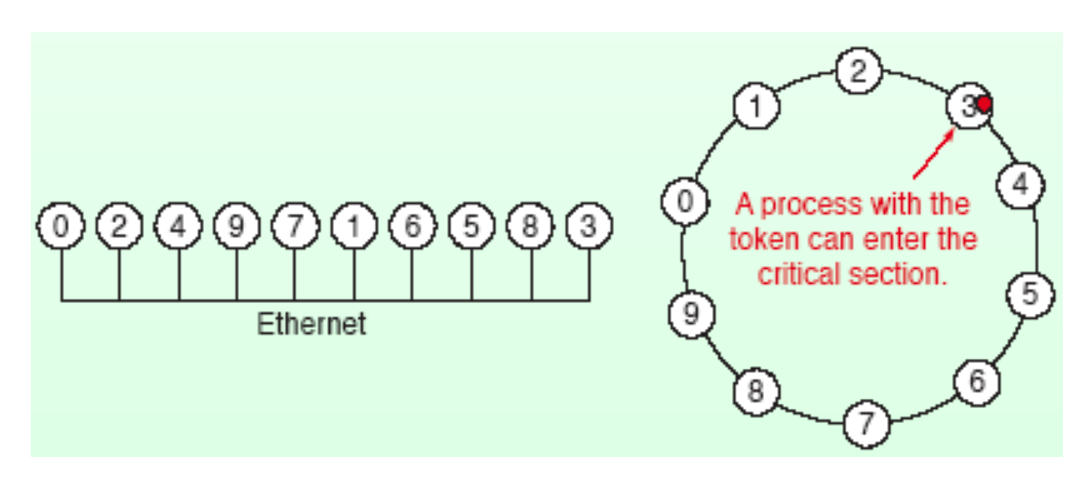
\includegraphics[width=0.7\linewidth]{screenshot035}
\caption{Token ring exclusion algorithm.}
\label{fig:screenshot035}
\end{figure}

In this algorithm, the processes do not suffer from starvation. Before attempting to enter a critical section, a process's waiting is bounded by the duration required for all other processes to enter and exit the critical section.

However, if a token is lost for some reason, another token must be generated. Detecting a loss of token is difficult as there is no upper bound for the time required for a token to traverse the ring. If a process crashes, the ring must be reconstructed.

\subsection{Mutual Exclusion Algorithm Comparison}
Based on this, a comparison can be drawn between the three algorithms.

For each entry/exit of a critical section, the centralised algorithm requires $3$ messages to be exchanged, the distributed algorithm requires $2(n-1)$ messages to be exchanged, and the ring algorithm requires $2$ messages to be exchanged.

Additionally, all three algorithms have reliability concerns. For a centralised system, the coordinator can crash. For a distributed system, any process crashing will break the system. For a token ring system, the loss of the token or a process crashing will result in disruption of the system while the ring is rebuilt.

\subsection{Group Mutual Exclusion}
In the group mutual exclusion problem, which generalizes mutual exclusion, processes choose a \textit{session} when they want entry to the Critical Section (CS); processes are allowed to be in the CS simultaneously given that they request the same session. This is illustrated in \autoref{fig:screenshot036}.

\begin{figure}
\centering
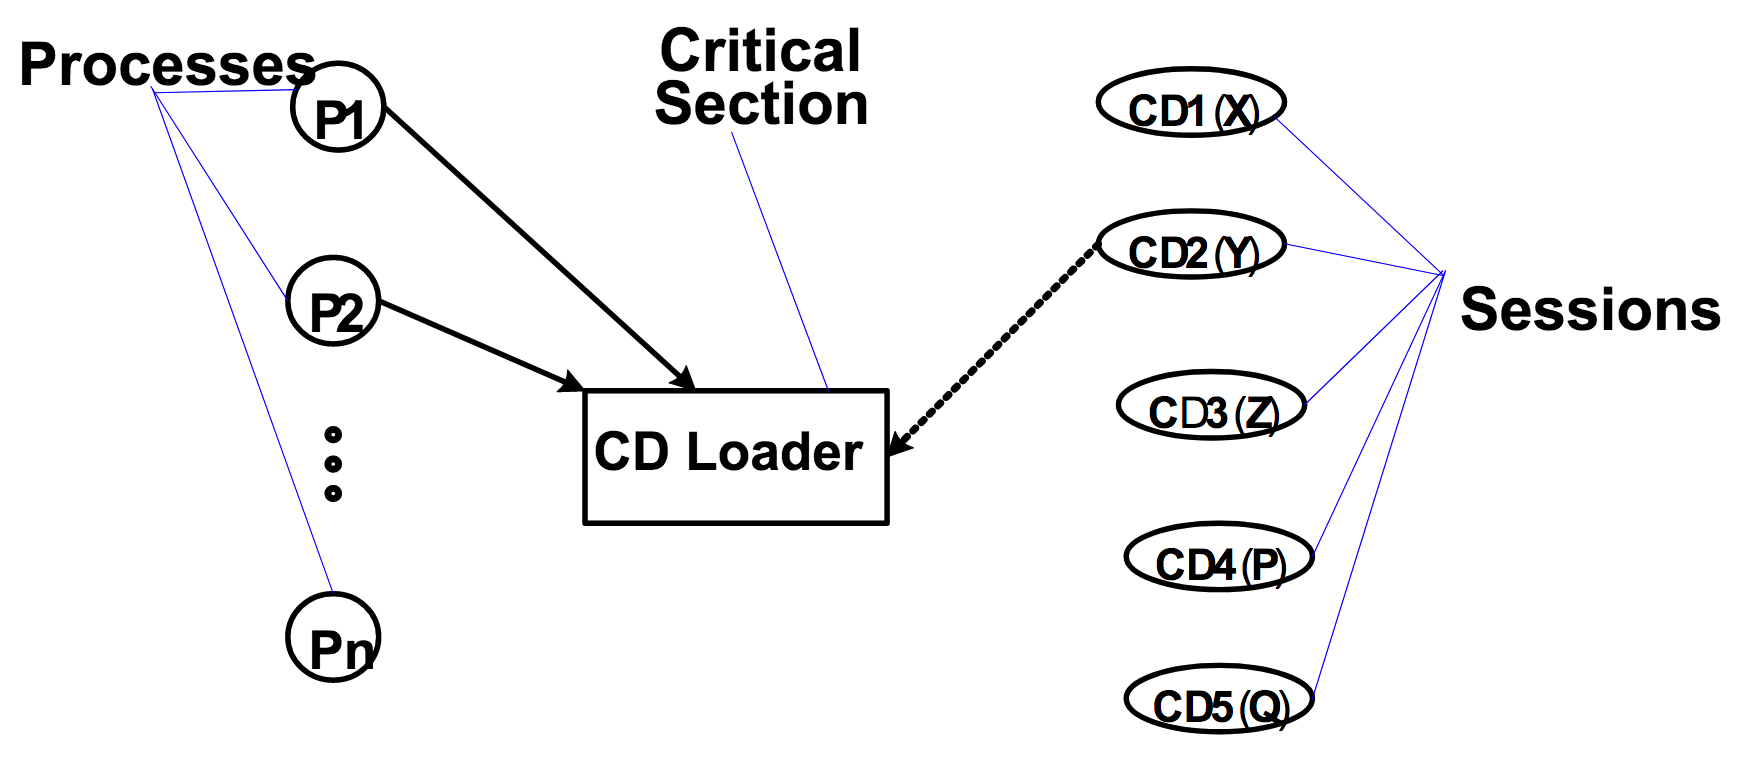
\includegraphics[width=0.7\linewidth]{screenshot036}
\caption{Group mutual exclusion problem.}
\label{fig:screenshot036}
\end{figure}

This problem is applicable to Computer Supported Cooperative Work (CSCW), wireless applications, improving the quality of services of an Internet server (i.e. by grouping requests for the same service), and more.

\section{Deadlocks}
A \textit{deadlock} is a condition where a process cannot proceed because it needs to obtain a resource held by another process and it itself is holding a resource that the other process needs. 

There are two types of deadlock to consider:
\begin{itemize}
\item \textbf{Communication deadlock} occurs when process A is trying to send a message to process B, which is trying to send a message to process C which is trying to send a message to A
\item \textbf{Resource deadlock} occurs when processes are trying to get exclusive access to devices, files, locks, servers, or other resources.
\end{itemize}

These will not be differentiated between as a communication channel can be considered to be a resource without loss of generality, which allows a communication deadlock to be treated as a resource deadlock.

There are four conditions that must be met for deadlock to occur:
\begin{itemize}
\item \textbf{Mutual exclusion}: A resource can be held by at most one process.
\item \textbf{Hold and wait}: Processes that already hold resources can wait for another resource. 
\item \textbf{Non-preemption}: A resource, once granted, cannot be taken away from a process. 
\item \textbf{Circular wait}: Two or more processes are waiting for resources held by one of the other processes. 
\end{itemize}

\subsection{Modelling}
A system with potential deadlocks can be modelled using a directed graph called a \textit{resource allocation graph}. In this graph, both the sets of nodes and edges are partitioned into two types, creating the graph elements seen in \autoref{fig:screenshot037}:
\begin{itemize}
\item \textbf{Process nodes}: $P_1, P_2, P_3$
\item \textbf{Resource nodes}: $R_1, R_2, R_3$
\item \textbf{Assignment edges}: $(R_1, P_1)$, $(R_1, P_3)$
\item \textbf{Request edges}: $(P_1, R_2), (P_2, R_1)$
\end{itemize}

\begin{figure}
\centering
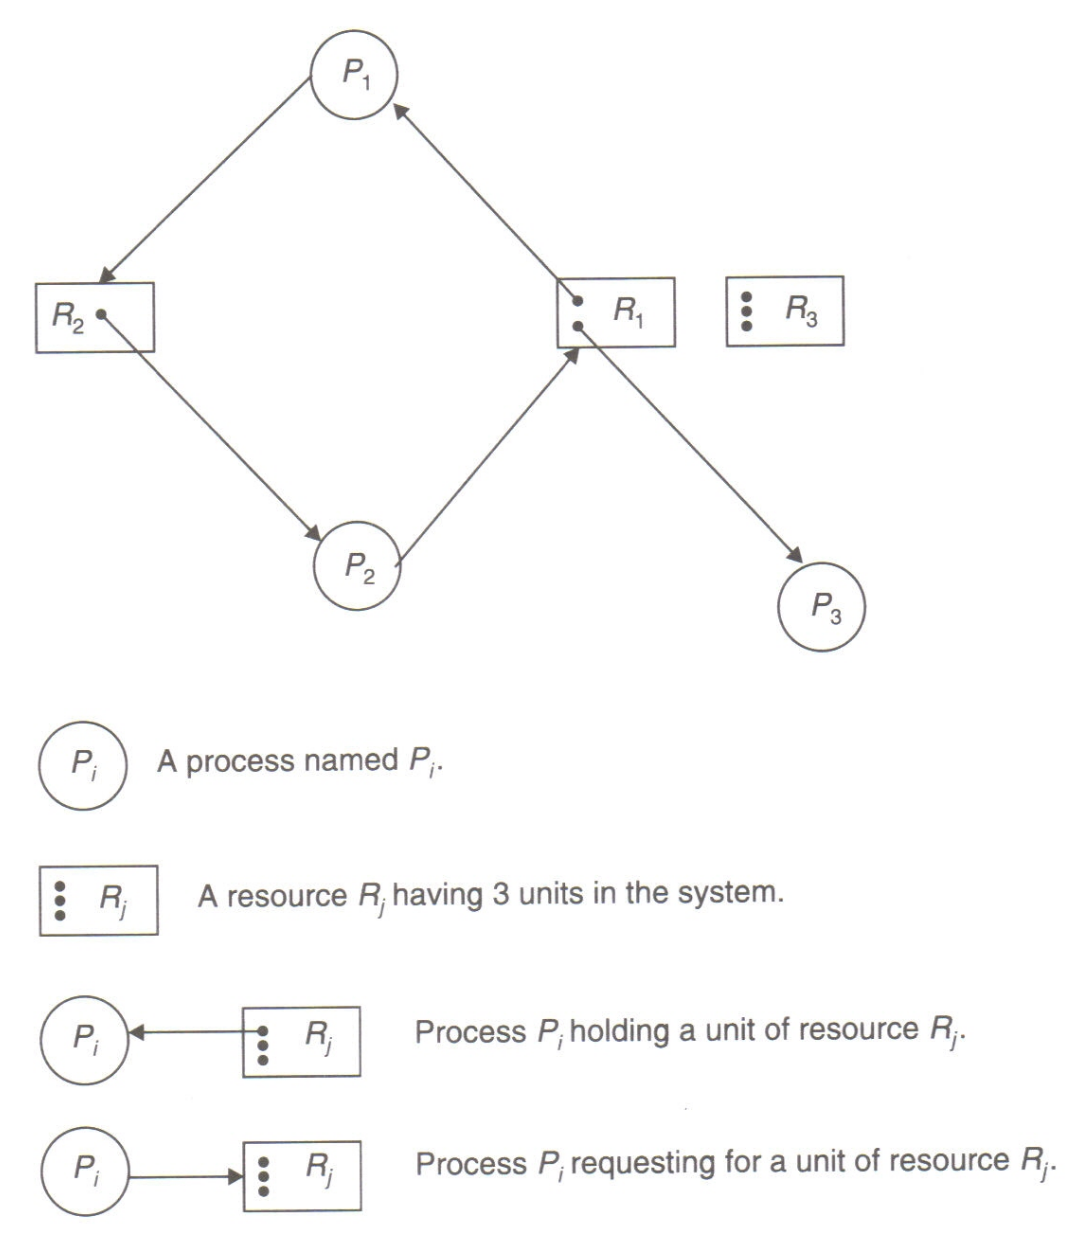
\includegraphics[width=0.6\linewidth]{screenshot037}
\caption{Resource allocation graph.}
\label{fig:screenshot037}
\end{figure}

A \textit{cycle} in the resource allocation graph, assuming that there is only one copy of all resources, is a necessary condition for a deadlock to exist; this can be seen in \autoref{fig:screenshot038}.

\begin{figure}
\centering
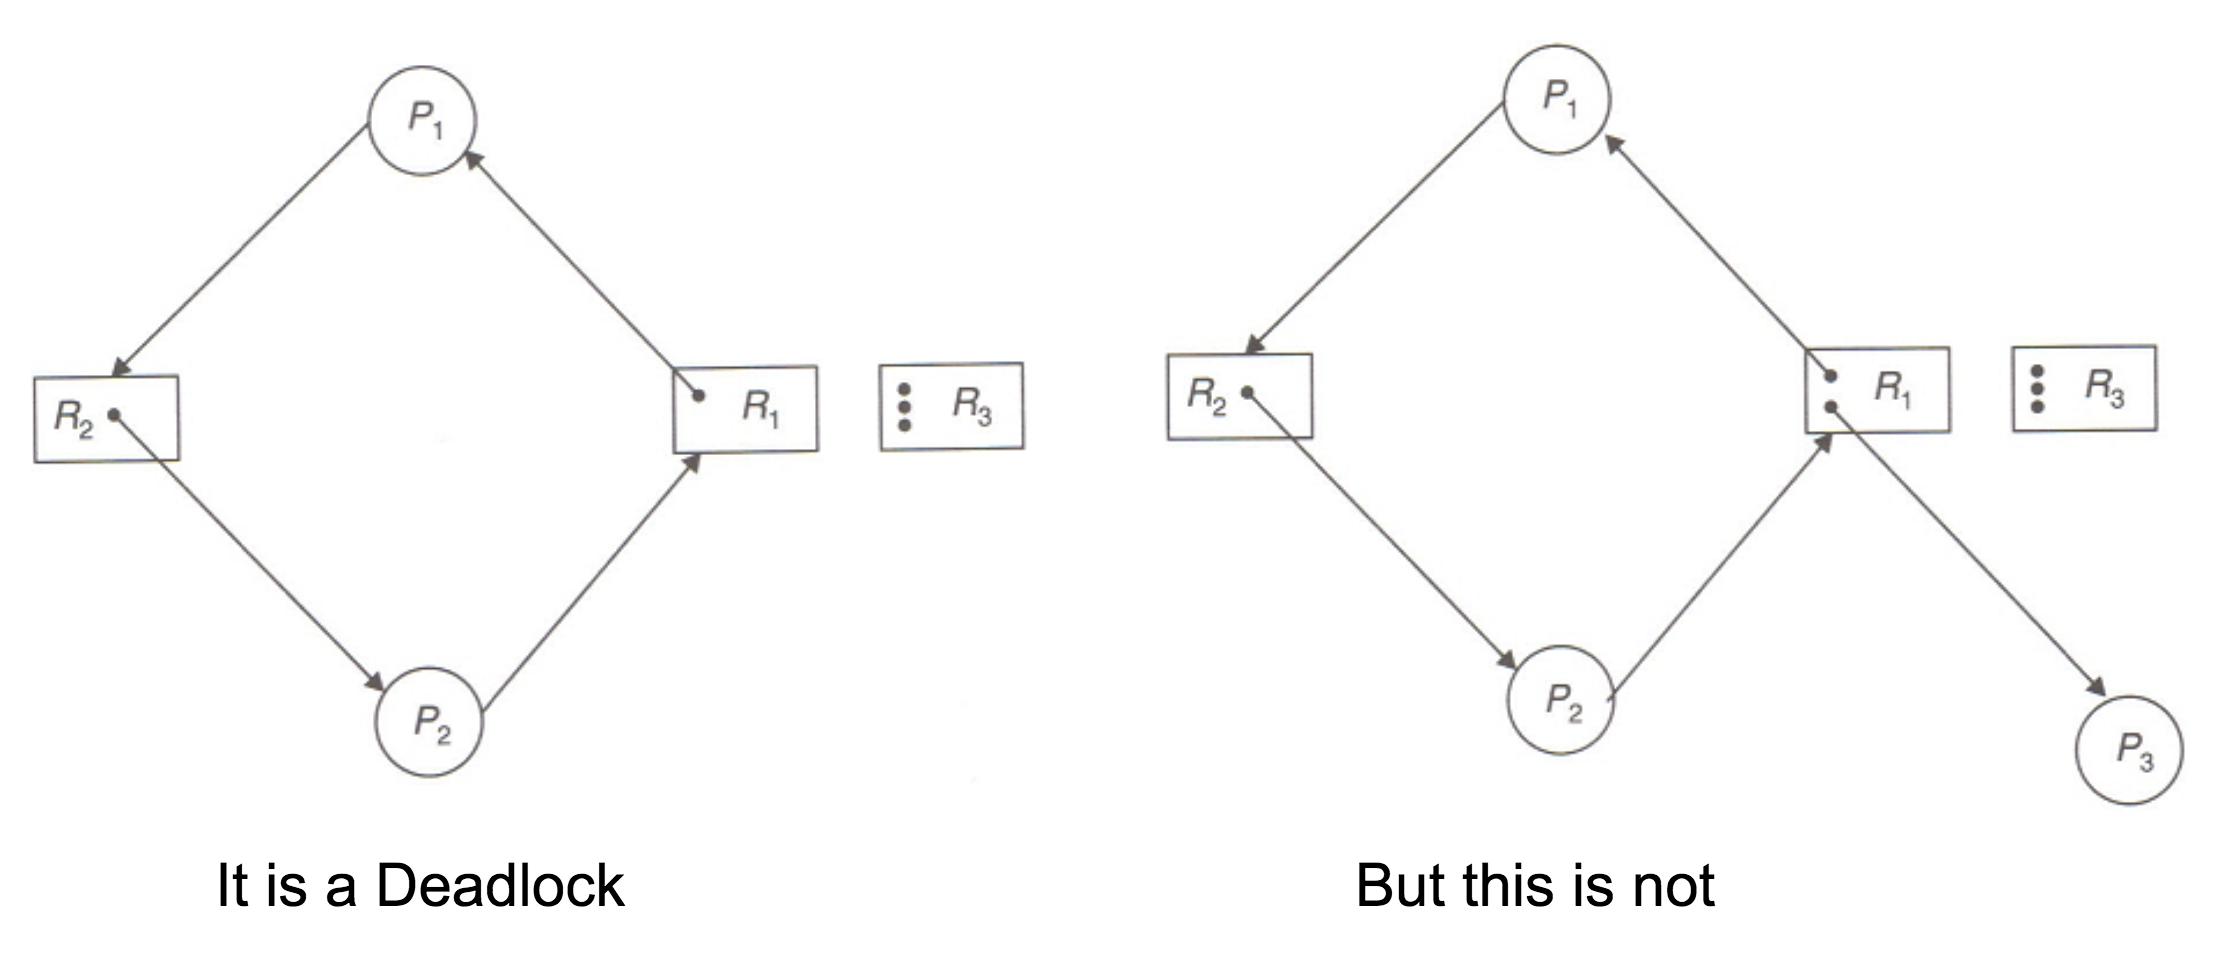
\includegraphics[width=0.6\linewidth]{screenshot038}
\caption{A cycle in the resource allocation graph.}
\label{fig:screenshot038}
\end{figure}

If there are multiple copies of some resources, then a \textit{knot} is required for deadlock to exist. A knot in a directed graph is a collection of vertices and edges with the property that every vertex in the knot has outgoing edges, and all outgoing edges from vertices in the knot terminate at other vertices in the knot. This is illustrated in \autoref{fig:screenshot039}.

\begin{figure}
\centering
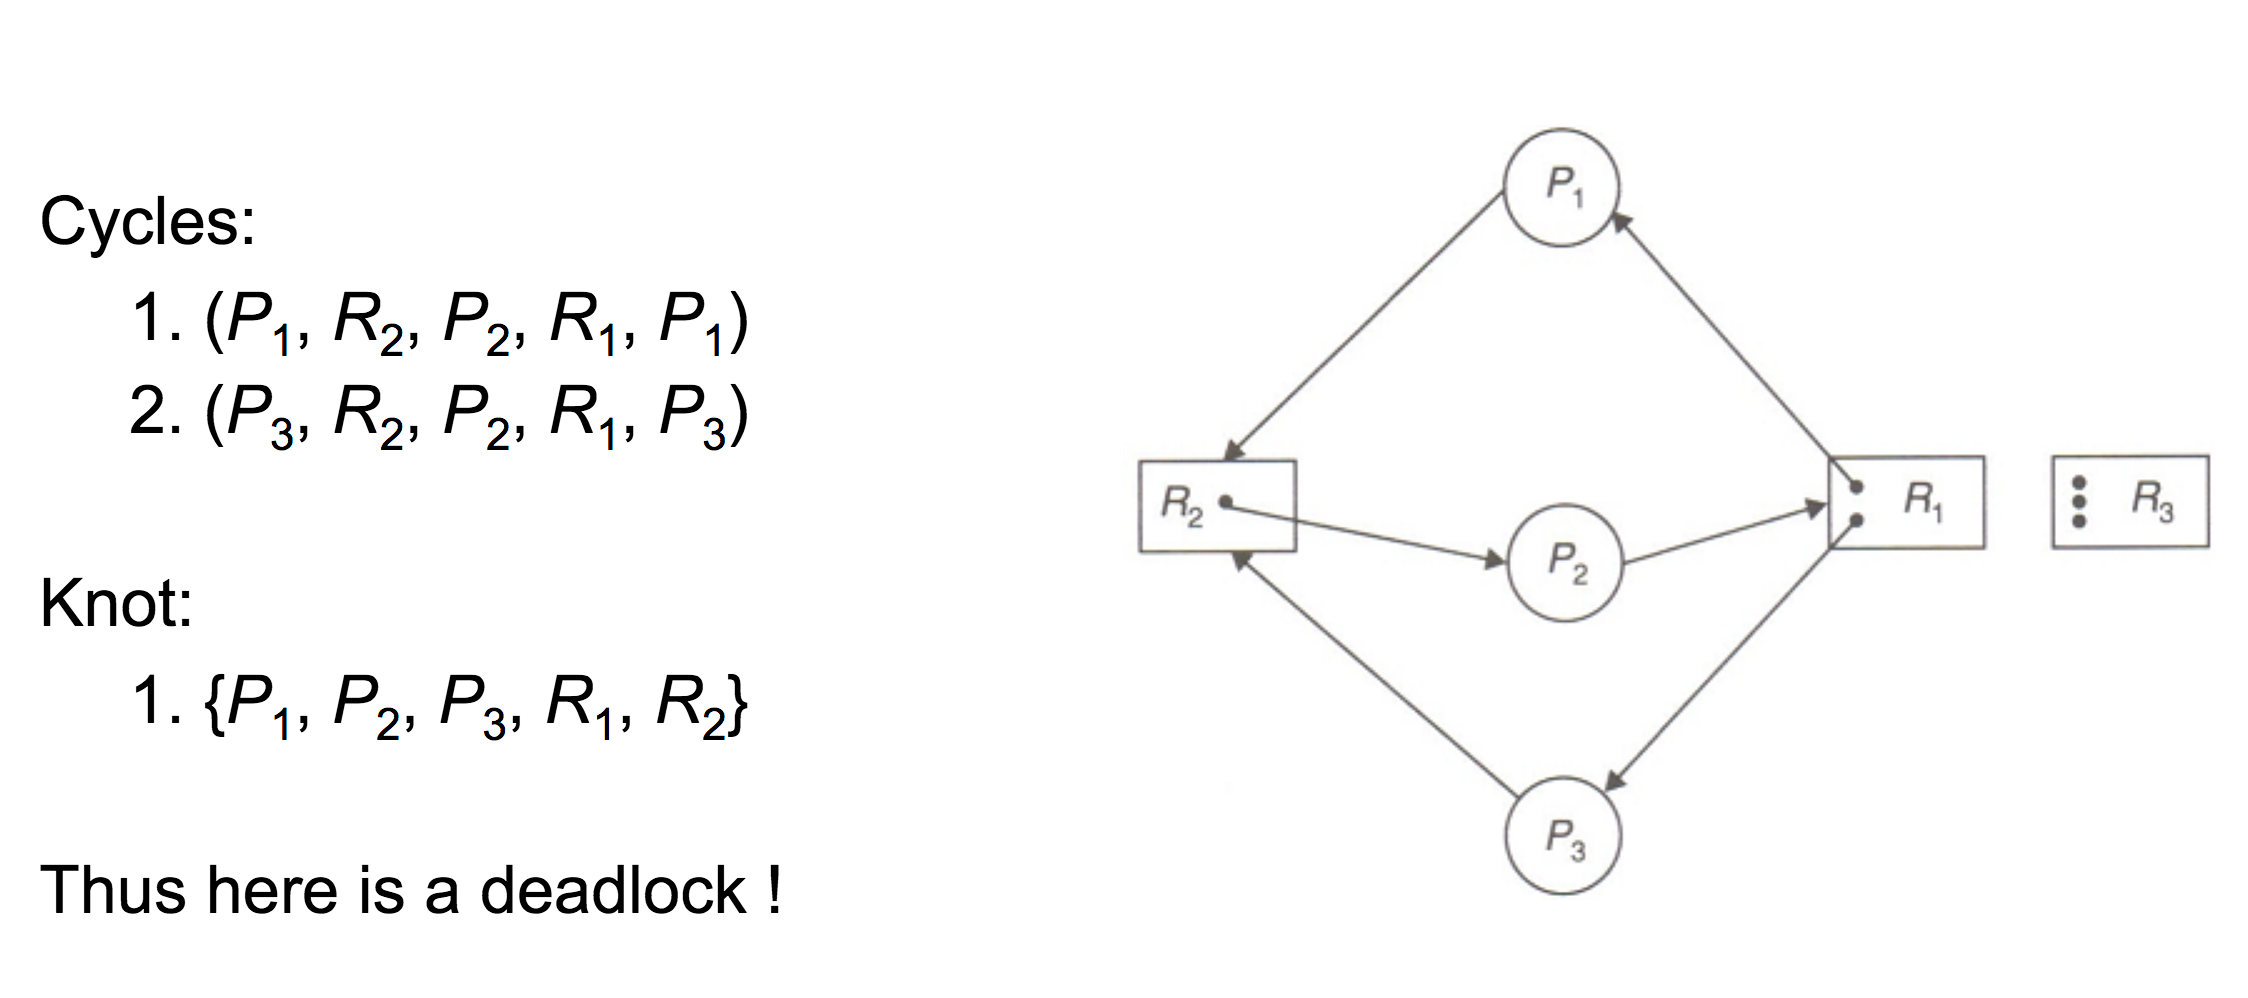
\includegraphics[width=0.6\linewidth]{screenshot039}
\caption{Deadlocks through cycles and knots.}
\label{fig:screenshot039}
\end{figure}

When there is only a single unit of each type of resource in the resource allocation graph, the graph can be simplified into a wait-for graph. This is done by removing the resource nodes and collapsing the appropriate edges. This is shown in \autoref{fig:screenshot040}.

\begin{figure}
\centering
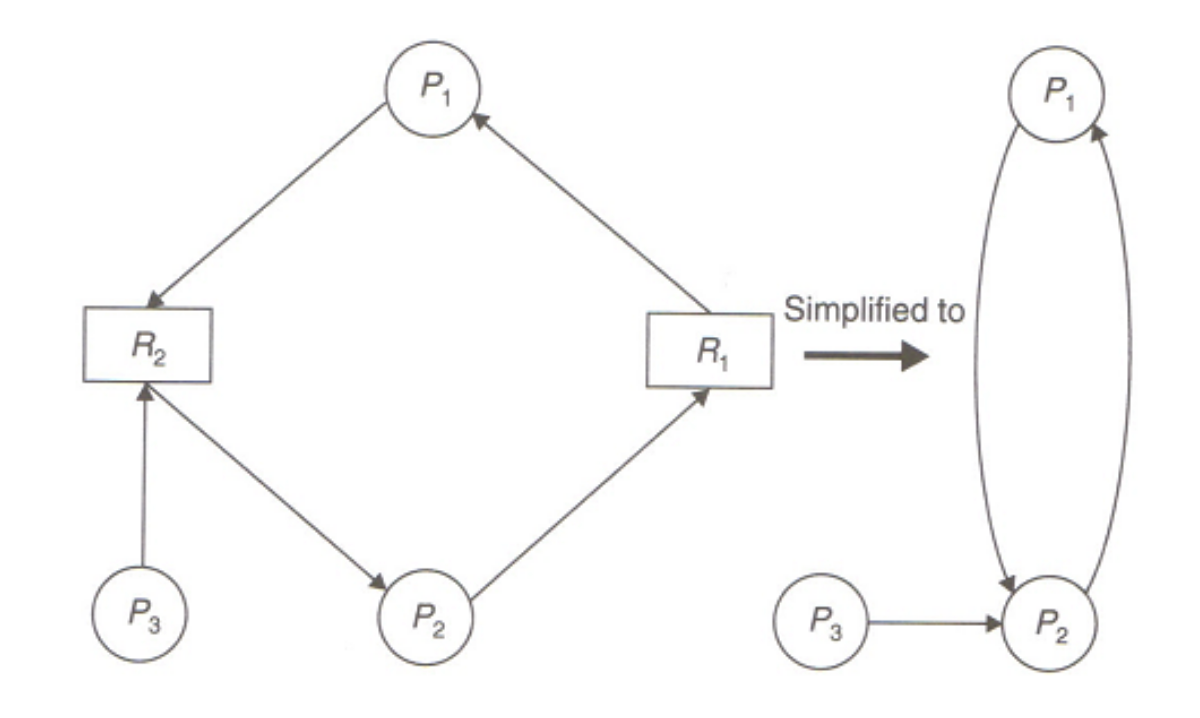
\includegraphics[width=0.7\linewidth]{screenshot040}
\caption{Resource allocation graph converted to wait-for graph.}
\label{fig:screenshot040}
\end{figure}

\section{Handling Deadlocks}
\subsection{Ostrich Algorithm}
Ignore the deadlock problem, bury your head in the sand, and pretend that everything is fine. \footnote{This doesn't actually work most of the time, y'know?}

\begin{figure}[h]
\centering
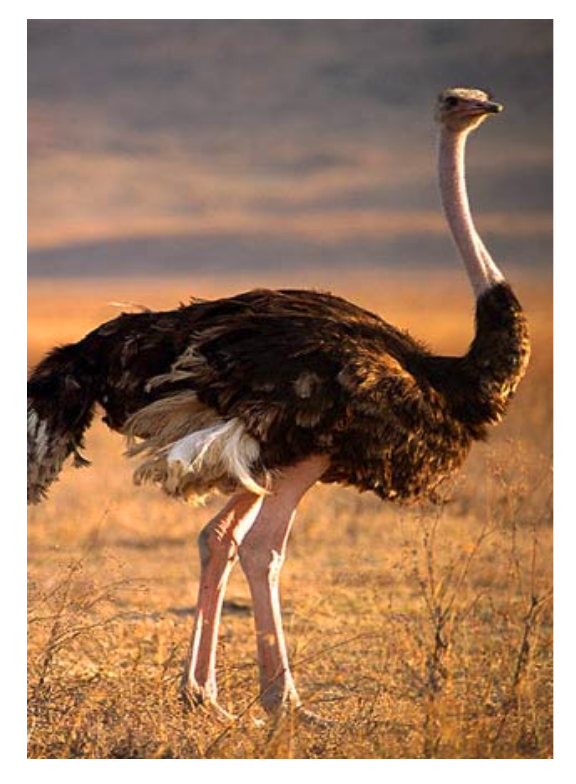
\includegraphics[width=0.7\linewidth]{screenshot041}
\caption{An ostrich.}
\label{fig:screenshot041}
\end{figure}

\pagebreak
\subsection{Detection}
Preventing or avoiding deadlocks can be difficult. Detecting them is easier. When a deadlock is detected, either kill off one or more processes (annoying users), or if the system is based on atomic transactions abort one or more transactions.

Transactions are generally designed to withstand being aborted. The system is restored to the state it was in before the transaction began, allowing the transaction to start a second time. As resource allocation in the system may be different, the transaction may succeed.
\subsubsection{Centralised deadlock detection algorithm}
The aim of the algorithm is to imitate the non-distributed algorithm through a coordinator, as seen in \autoref{fig:screenshot042}. Each machine maintains a resource graph for its processes and resources. A central coordinator maintains a graph for the entire system, and a message can be sent to the coordinator each time an arc is added or deleted by a machine. The list of arc adds/deletes can be sent periodically.

\begin{figure}
\centering
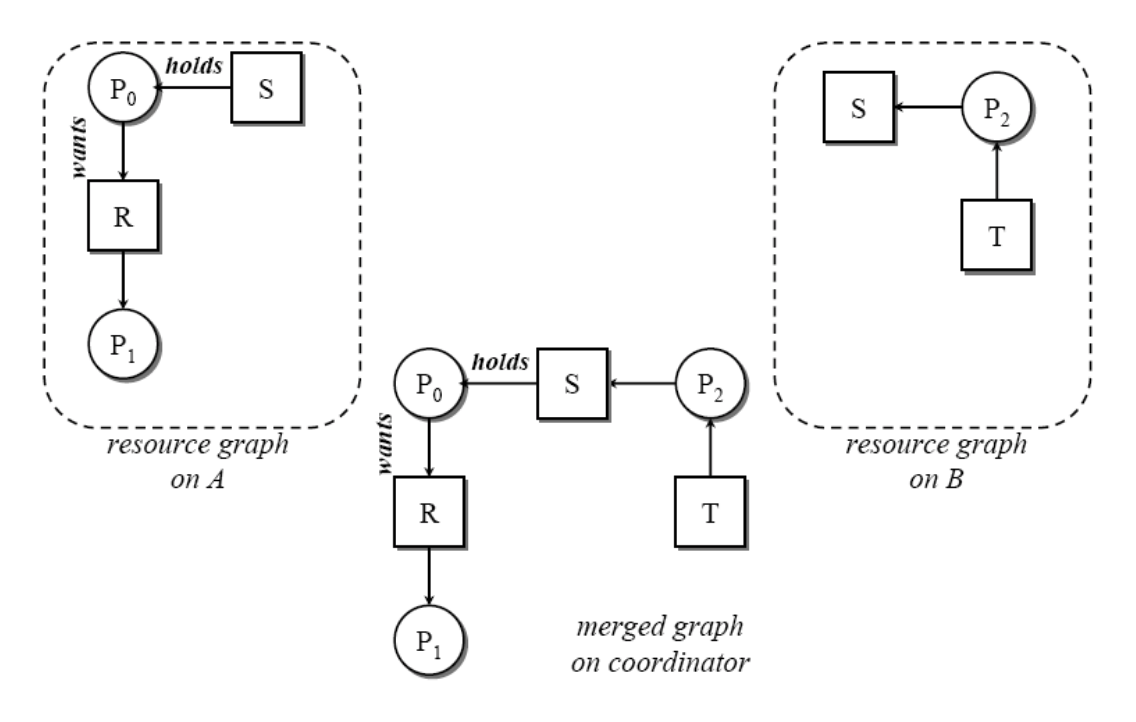
\includegraphics[width=0.7\linewidth]{screenshot042}
\caption{Diagram of the centralised deadlock algorithm.}
\label{fig:screenshot042}
\end{figure}

However, this algorithm is susceptible to \textit{false deadlock}. Examine \autoref{fig:screenshot043}. If $P_1$ releases a resource $R$ and then asks for a resource $T$ from $P_2$, the coordinator may receive the message about waiting prior to the message about releasing. The coordinator will then end up construct a graph with a cycle, resulting in a detection of a deadlock.

\begin{figure}
\centering
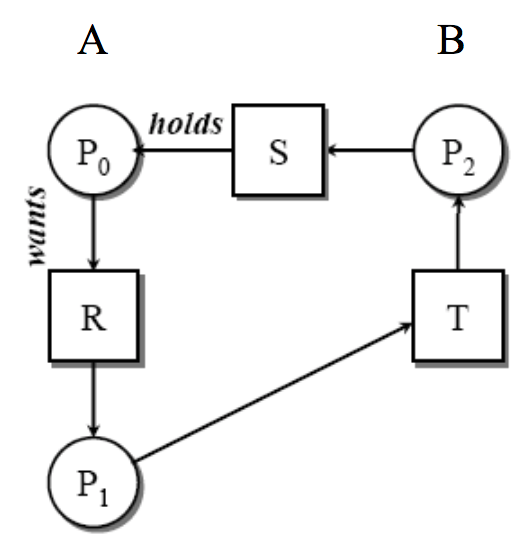
\includegraphics[width=0.4\linewidth]{screenshot043}
\caption{False deadlock in the centralised deadlock detection algorithm.}
\label{fig:screenshot043}
\end{figure}

This can be mitigated by enforcing global time ordering on all machines, or by using a reliable communication method to ask each machine whether it has any release messages prior to making a deadlock detection claim.

\subsubsection{Chandy-Misra-Haas algorithm}
The CMH algorithm is a distributed algorithm for deadlock detection, illustrated in \autoref{fig:screenshot044}. Processes can request multiple resources at once. Some processes wait for local resources. Some processes wait for resources on other machines. The algorithm is invoked when a process has to wait for a resource.

When a process has to wait for a resource, a probe message is generated. This message contains 3 fields: process that was just blocked, the process sending the message, and the process to whom it is being sent.

When the probe message arrives, the recipient checks to see if it is waiting for any processes. If it is not, the message is ignored. If it is, the message is updated; the second field is replaced with its own process number, and the third field is replaced with the number of the process it is waiting for. The message is then sent to each process on which the recipient is blocked o.

If a message goes all the way around and comes back to the original sender, a cycle exists, and thus deadlock has occurred.

\begin{figure}[h]
\centering
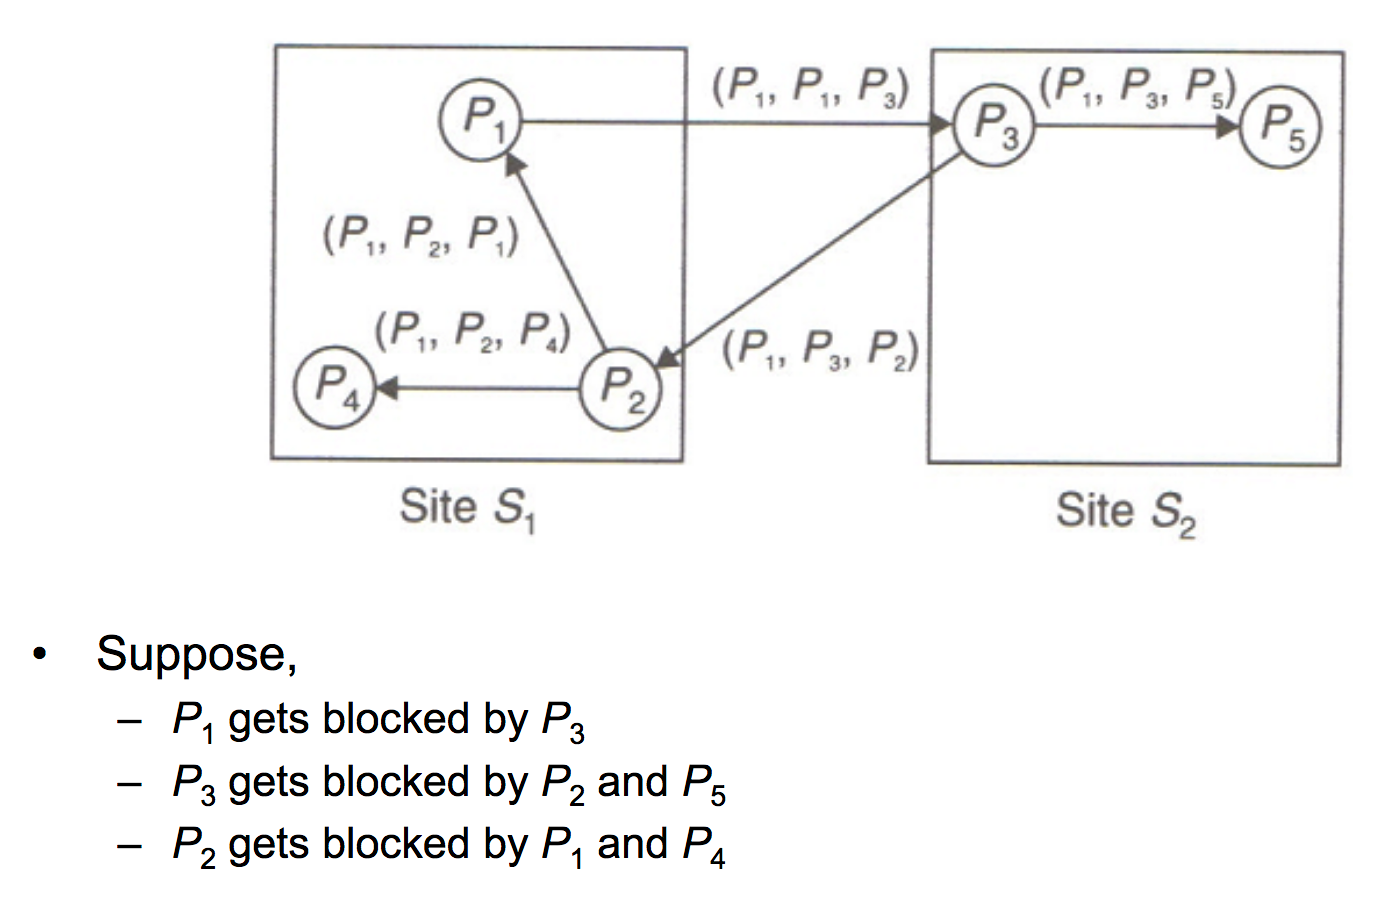
\includegraphics[width=0.5\linewidth]{screenshot044}
\caption{Chandy-Misra-Haas algorithm diagram.}
\label{fig:screenshot044}
\end{figure}

\subsubsection{Recovery After Detection}
After deadlock has been detected, several measures can be used. The operator can be asked to intervene, processes can be autonomously terminated, or process state can be rolled back. These each have their own advantages and disadvantages, especially with regards to performance and minimisation of frustration for the operator.

Additionally, recovery may involve other issues, such as minimisation of recovery cost and the prevention of starvation. \footnote{These are left as an exercise to the reader to contemplate.}
